%% ----------------------------------------------------------------------------
% BIWI SA/MA thesis template
%
% Created 09/29/2006 by Andreas Ess
% Extended 13/02/2009 by Jan Lesniak - jlesniak@vision.ee.ethz.ch
%% ----------------------------------------------------------------------------
\newpage
\chapter{Materials and Methods}
\section{Loss Guided Diffusion}
Both, Choi et al. and Lugmayr et al. make use of unconditional DDPMs for image-guided diffusion for the tasks of image translation in the former and in-painting in the latter.~\autocite{choi2021ilvr,lugmayr2022repaint} Similarly, classifier guidance or CLIP-guidance can be used to condition unconditional DDPMs to produce samples of a specific class or to match a prompt.~\autocite{dhariwal2021diffusion} Both approaches can be combined into a flexible framework that allows the reverse diffusion process to be conditioned on any data consistency term.

\subsection{MAP Estimation for Inverse Problems}
Image reconstruction tasks, that make use of a prior over the desired reconstructed image, can be formulated as a MAP (maximum-a-posteriori) estimation problem
\begin{equation}
    \hat{x}_{MAP} = \argmax_x p(x|s) = \argmax_x \frac{p(s|x)p(x)}{p(s)}
\end{equation}
where $s \sim p(s)$ is the evidence that is provided by the measured signal, $p(x)$ is a prior on the desired reconstruction and the likelihood term $p(s|x)$ enforces a data consistency between the measured signal and the true distribution. Since maximizing $p(x|s)$ is the same as maximizing $\log(x|s)$ and $p(s)$ is independent of $\theta$, we can separate the product into a sum.
\begin{align}
    \hat{x}_{MAP} & = \argmax_x \log p(x|s)             \\ & = \argmax_x \log{\frac{p(s|x)p(x)}{p(s)}} \\
                  & = \argmax_x \log p(s|x)p(x)         \\
                  & = \argmax_x \log p(s|x) + \log p(x)
\end{align}
Such problems can be optimized using iterative optimization schemes like gradient ascent
\begin{align}
    \label{eq:mapestimation}
    x_{i+1} = x_{i} + \lambda_1 \nabla_{x_i} \log p(s|x_i) + \lambda_2 \nabla_{x_i} \log p(x_i)
\end{align}
with $\lambda_{1,2}$ being step sizes or weights assigned to the two terms allowing the reconstruction to put more trust in either the data consistency or the prior.

Maximizing $p(s|x)$ and $p(x)$ is in practice usually reformulated as a minimization problem that optimizes for smallest error between prediction and acquisition $\mathcal{L}(s, x)$ and enforces certain regularizers (priors) on $x$ by minimizing $\mathcal{R}(x)$. An example for MRI reconstruction could include minimizing a mean-squared-error between predicted k-space $\mathcal{F}(x)$ and acquired k-space $s$, while also minimizing the total variation in the image.~\autocite{RUDIN1992259}
\begin{equation}
    \hat{x}_{MAP} = \argmin_x \mathcal{L}(s, x) + \mathcal{R}(x) = \argmin_x \frac{1}{n}||\mathcal{F}(x) - s||_2^2 + TV(x)
\end{equation}

\subsection{DDPMs as Priors}
\label{sec:lossguidance}
DDPMs approximate a data distribution over training images $p(x)$ and by the score-based formulation, they do so by learning to approximate gradients of this marginal likelihood.~\autocite{song2020generative} As already mentioned in~\ref{sec:classifierguidance}, sampling a DDPM therefore equals to starting in a random position and taking gradient ascent steps in the direction of maximizing $p(x)$ or $\log p(x)$.
\begin{equation}
    \label{eq:ddpmiteration}
    x_{t-1} = x_{t} + \nabla_{x_t} \log p(x_t)
\end{equation}
Comparing this to Eq.~\ref{eq:mapestimation} it is easy to see that this is the same as maximizing for a prior in a reconstruction task and we can introduce a data consistency that works similarly to classifier-guidance~\autocite{dhariwal2021diffusion}, but makes the reverse diffusion process converge to acquired data instead of an easily-classified image.
\begin{align}
    \hat{x} & = \argmax_x \log p(x) + \log p_{\theta}(c|x)        &  & \text{(classifier-guidance)}       \\
            & = \argmax_x \log p(x) + \log p(s|x)                 &  & \text{(data-consistency guidance)} \\
            & = \argmax_x \log p(x) + \argmin_x \mathcal{L}(s, x) &  & \text{(for $\mathcal{L} \geq 0$)}  \\
\end{align}
The constraint $\mathcal{L} \geq 0$ is true for the usual distance-based loss functions like mean-squared-error or the $L_1$ loss. A step in the iterative process has the following form and this algorithm will from now on be termed \textit{loss-guidance}.
\begin{equation}
    x_{t-1} = x_{t} + \nabla_{x_t} \log p(x_t) - \nabla_{x_t} \mathcal{L}(s, x)
\end{equation}
The formulation used for the task of reconstructing undersampled MRI used an MSE loss between the predicted $\mathcal{F}(x_t)$ and acquired k-space $s_0$
\begin{equation}
    x_{t-1} = x_{t} + \nabla_{x_t} \log p(x_t) - g \cdot \nabla_{x_t} \frac{1}{\sum_n \mathcal{M}}||\mathcal{M} \circ \mathcal{F}(x_t) - s_0||_2^2
\end{equation}
where $g$ will be termed the \textit{guidance factor} and the MSE is not scaled by the number of pixels in the image, but by the number of non-zero elements of the mask. This is done in order to compare guidance factors among masks with different accelerations. Similar to $\lambda_{1,2}$ in Eq.~\ref{eq:mapestimation}, the guidance factor $g$ can be used to balance adherence of the outcome between prior and data consistency.

\section{Frequency Replacement}
\label{sec:freqreplacement}
As already stated in~\ref{sec:imageguidance}, Choi et al. guide the diffusion process by substituting low frequency content of a desired latent representation with the low-frequencies of the predicted latent space. Since they use linear filters, the equation can be reformulated as
\begin{align}
    \label{eq:ilvr}
    x_{t} & = \phi(s_{t}) + (I - \phi) (\hat{x}_{t})        \\
          & = \hat{x}_{t} + \phi(s_{t}) - \phi(\hat{x}_{t}) \\
          & = \hat{x}_{t} + \phi(s_{t} - \hat{x}_{t})       \\
          & = \hat{x}_{t} - \phi(\hat{x}_{t} - s_{t})
\end{align}
where $\phi$ is a linear filter operation and $s_t$ is obtained by using the forward process on the target image.~\autocite{choi2021ilvr} With knowledge of the gradient of the MSE
\begin{align}
    \text{MSE}              & = \frac{1}{N} (x - s)^T (x - s) \\
    \nabla_{x_t} \text{MSE} & = \frac{2}{N} (x - s)
\end{align}
the frequency replacement can actually be interpreted as locally approximating the gradient of the $\nabla_{x}\text{MSE}(\phi(s), \phi(x_{t}))$ in $s=s_t$ and taking a step in that direction, which is very similar to the loss guidance from earlier.

Similarly, Lugmayr et al. use a replacement strategy, which can be reformulated to the structure from Choi et al.
\begin{align}
    \label{eq:repaint}
    x_{t} & = \mathcal{M}(s_t) + \mathcal{M}^{-1}(\hat{x}_t)        \\
          & = \mathcal{M}(s_t) + (I - \mathcal{M})(\hat{x}_t)       \\
          & = \hat{x}_t - \mathcal{M}(\hat{x}_t) + \mathcal{M}(s_t) \\
          & = \hat{x}_t + \mathcal{M}(s_t - \hat{x}_t)
\end{align}
As one can see, the two approaches only differ in the type of linear operation applied, and are therefore easily adapted to the task of MRI reconstruction. This requires calculating $s_t$ from $s_0$ which can be done in image space as
\begin{equation}
    s_t = \mathcal{F}^{-1} \circ \mathcal{M} \circ \mathcal{F} (\sqrt{\bar{\alpha}_t} \mathcal{F}^{-1}(s_0) + \sqrt{1-\bar{\alpha}_t} \epsilon)
\end{equation}
or directly in k-space as
\begin{equation}
    \label{eq:kspaceforward}
    s_t = \mathcal{F}^{-1} \circ \mathcal{M} (\sqrt{\bar{\alpha}_t} s_0 + \sqrt{\frac{1-\bar{\alpha}_t}{2}} \epsilon).
\end{equation}
The scaling of the noise variance with factor $\frac{1}{2}$ in Eq.~\ref{eq:kspaceforward} was experimentally found and can be verified in Fig.~\ref{fig:kspacedistribution}. The complete formulation of the update step is therefore
\begin{align}
    x_{t} & = \hat{x}_t - \mathcal{F}^{-1}\circ\mathcal{M}\circ\mathcal{F}(\hat{x}_t) + \mathcal{F}^{-1} \circ \mathcal{M} \circ \mathcal{F} (s_t) \\
          & = \hat{x}_t + \mathcal{F}^{-1}\left(\mathcal{M} \circ \mathcal{F} (s_t) - \mathcal{M}\circ\mathcal{F}(\hat{x}_t)\right).
\end{align}

\section{Network Architecture}
\label{sec:networkarch}
The neural network is responsible for predicting the noise in an image and the UNet architecture has proven useful for estimating the noise in natural images, which is the context where DDPMs usually operate.~\autocite{ronneberger2015unet,ho2020denoising} The UNet implementation which was used in most experiments of this work is closely related to the original implementation by Ronneberger et al., which means that it is a fully convolutional architecture. This is in contrast to most other works, that make use of more sophisticated architectures that include Transformer-inspired self-attention layers for better global context awareness of the model and residual connections for faster convergence.~\autocite{vaswani2017attention,he2015deep} Saharia et al. did ablation studies on the self-attention layers and tried to replace them with other methods, such as local self-attention or dilated convolutions, but showed that the global self-attention increased both, mode coverage of the data distribution as well as sample fidelity.~\autocite{saharia2022palette} Fully convolutional architectures on the other hand have the advantage that, if trained appropriately, they can generalize to different image resolutions, which was the motivation behind using a fully convolutional network. Such training could be done on random crops of the training images, while sampling would happen in the full resolution. The created network was later modified to allow for the inclusion of self-attention layers, but the additional computational cost made it difficult to reach convergence in a reasonable time and the results from the fully convolutional architectures were deemed sufficient for the context of this work. Therefore the best network checkpoint, that was used in the conditioning studies of~\ref{sec:experimentsandresults}, uses the fully convolutional architecture as presented in Fig.~\ref{fig:unetconv}. This architecture sequentially increases the channels and decreases the resolution with a factor of 2 in the encoder and then upsamples the outputs of this bottleneck by incorporating additional local information through the use of skip-connections. Every block of the encoder does this by double-convolutions (without residual connections) and max-pooling, while the decoder uses transpose convolutions and double-convolutions for the upsampling. The network offers two possibilities of increasing the total amount of parameters: 1. Increasing the encoder depth, which is limited by the resolution of the training images; 2. Increasing the number of initial channels, which can for example be 64, 128 or 256. The exact network specifications can be found in Table~\ref{tab:unetlayers}.

Noise prediction is easier for the network if it is conditioned on the timestep of the training image. This conditioning is done by broadcasting a linear embedding of the Transformer-style time encoding (see Fig.~\ref{fig:timeencoding}) onto the feature dimension (channels).~\autocite{vaswani2017attention}
\begin{figure}
    \centering
    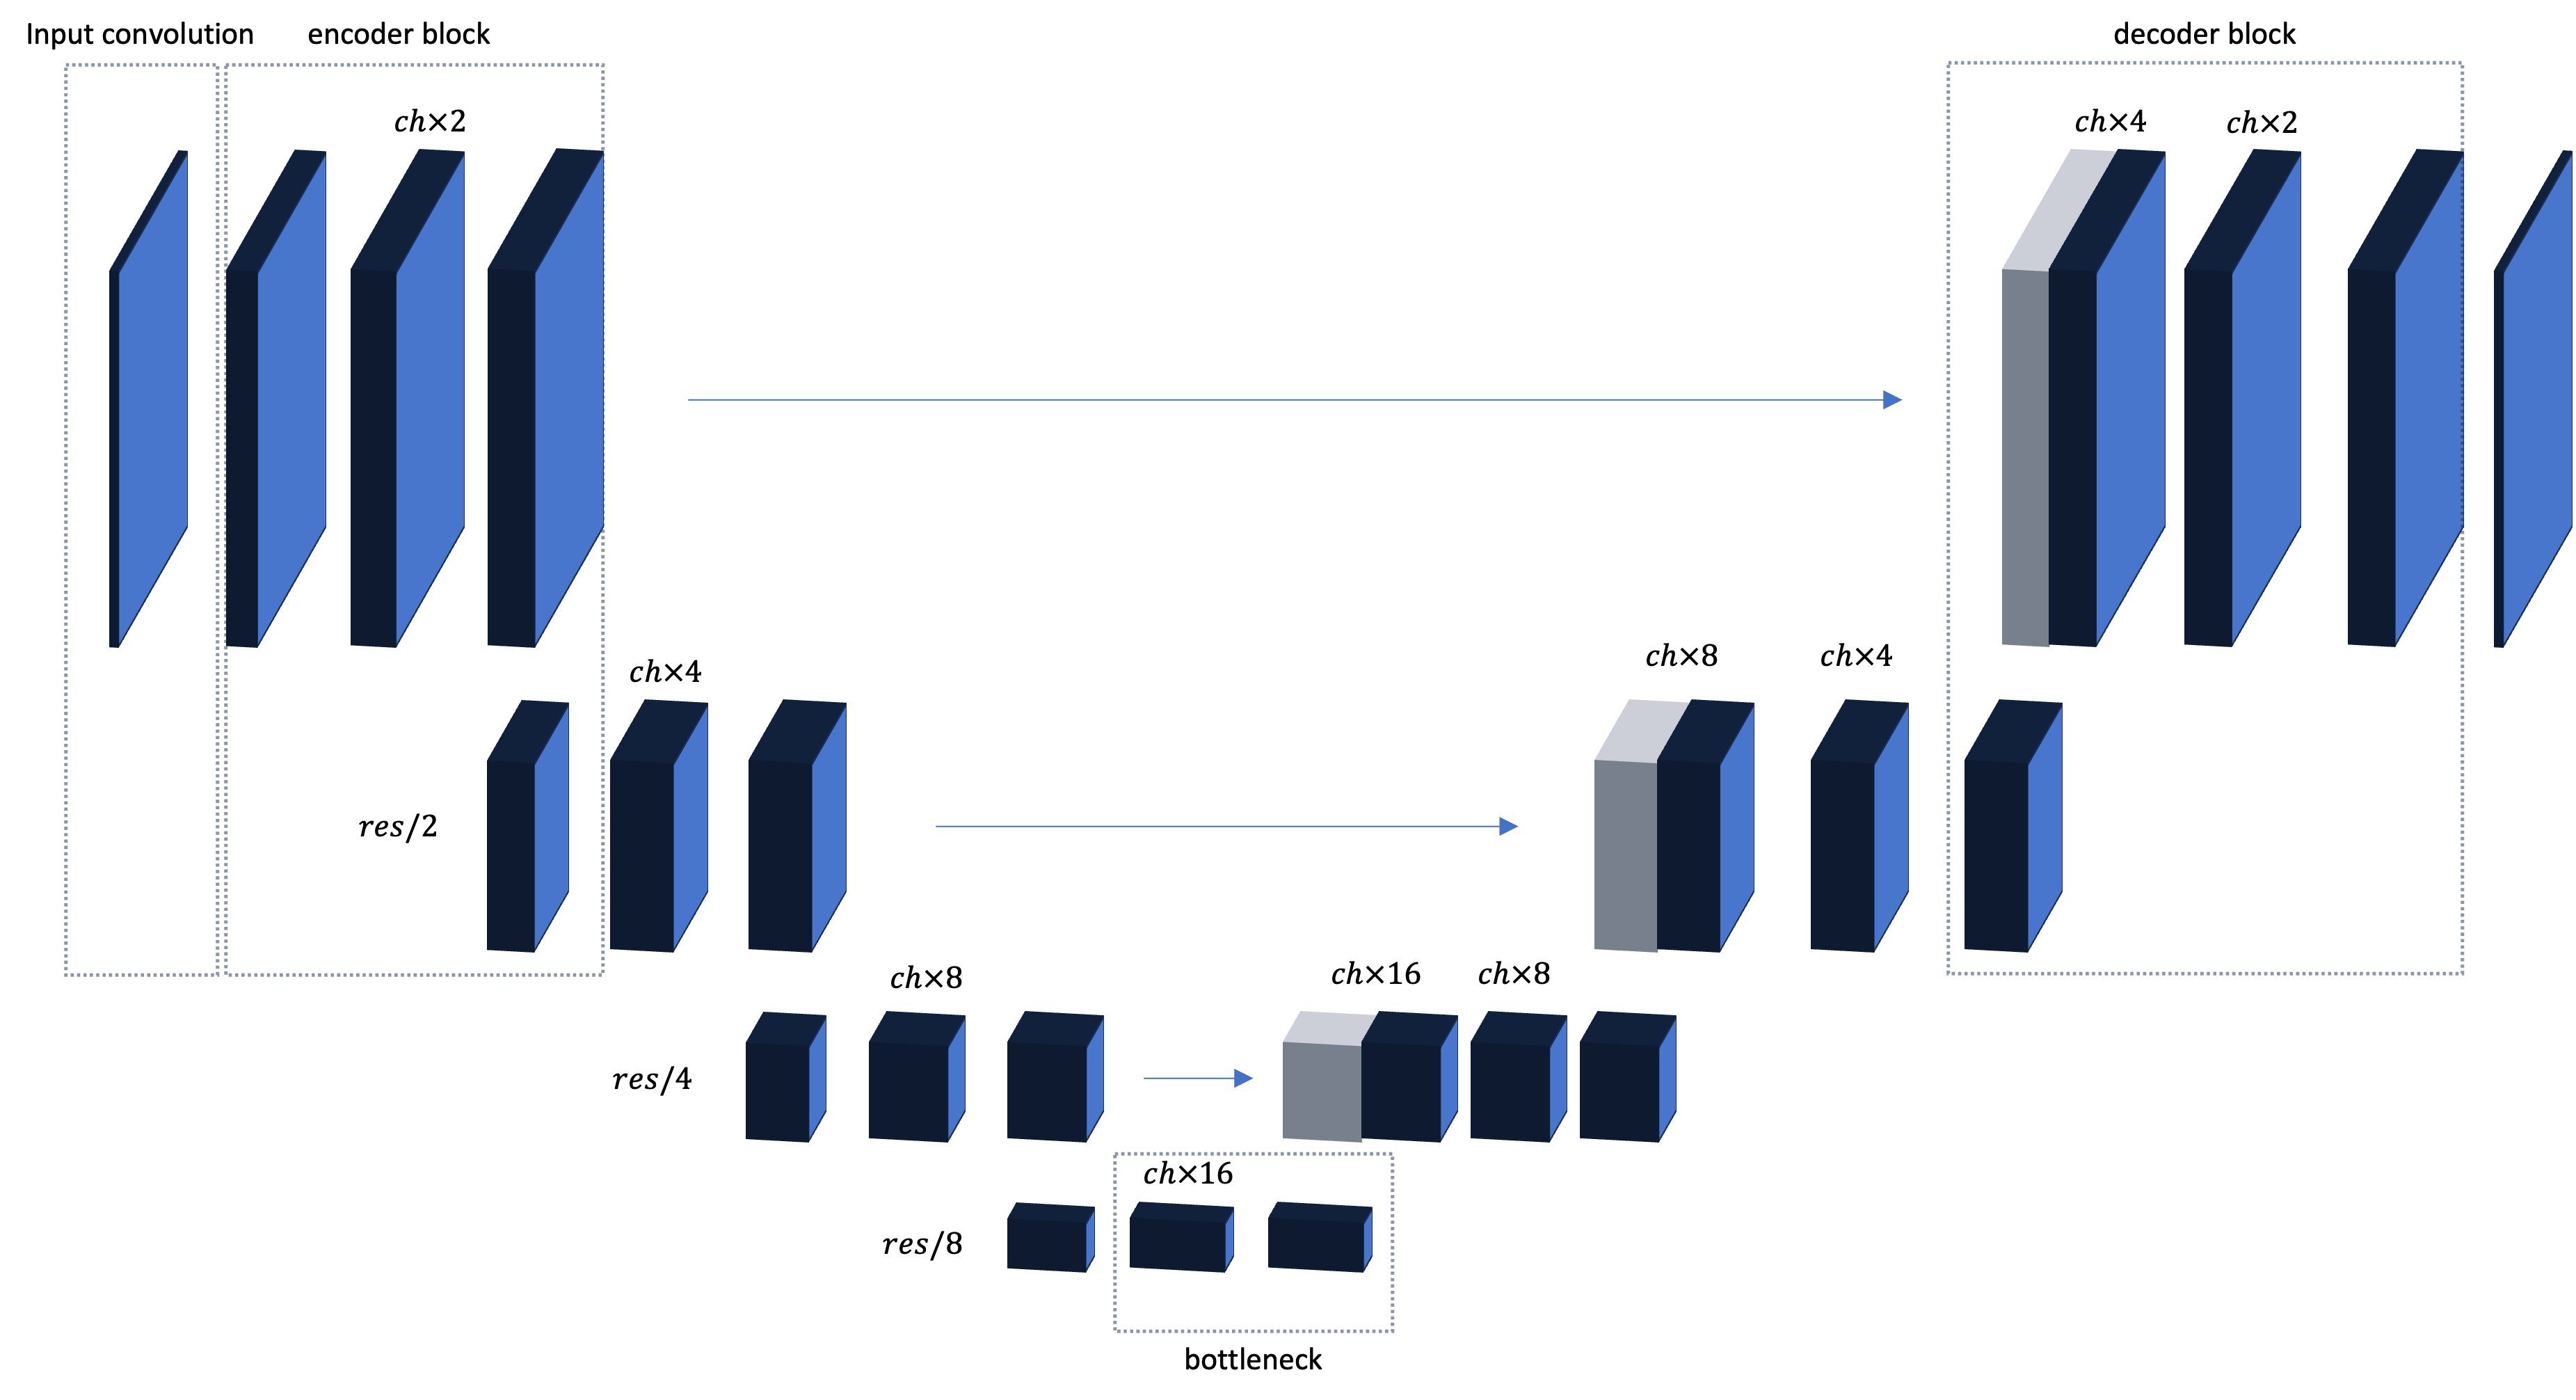
\includegraphics[width=.7\textwidth]{images/unet.png}
    \caption[Fully Convolutional UNet]{Fully Convolutional UNet architecture: An input convolution increases the channels to the number of base channels \textit{ch}. Consecutively a variable number of encoder blocks applies double convolutions and max pooling, before the decoder block applies transpose convolutions for upsampling and double convolutions to incorporate information from the skip connections. All double convolutions in the encoder and decoder further condition the model on the time encoding by broadcasting a time embedding onto the hidden layer, as illustrated in Fig.~\ref{fig:timeencoding}. At the end, the output convolution maps the output back to the original number of input channels.}
    \label{fig:unetconv}
\end{figure}

\begin{table}
    \centering
    \caption[Overview over UNet Architecture]{Overview over UNet Architecture.}
    \label{tab:unetlayers}
    \begin{tabular}{l l}
        \textbf{architecture part}     & \textbf{specification}                                                            \\
        \hline\hline
        base channels ($ch$)           & $2^n$, usually 64, 128, 256                                                       \\
        \hline base resolution ($res$) & $2^x \times 2^m$, usually square $64\times 64$ or $128\times 128$                 \\ \hline
        convolutional block            & convolution                                                                       \\ & batchnorm\\ & activation\\ & dropout                         \\
        \hline encoder block           & convolutional block ($ch \rightarrow ch\times 2$)                                 \\ & convolutional block ($ch\times 2 \rightarrow ch\times 2$) \\ & max pool ($res\rightarrow res/ 2$) \\
        \hline decoder block           & transpose convolution ($res\times 2\rightarrow res$, $ch\times 2 \rightarrow ch$) \\ & batchnorm\\ & activation\\ & dropout \\ & skip connection stack ($ch \rightarrow ch\times 2$) \\ & convolutional block ($ch\times 2 \rightarrow ch$)\\
        \hline bottleneck              & convolutional block ($ch \rightarrow ch\times 2$)
    \end{tabular}
\end{table}


\section{Slowing Down, Short-Grained Resampling \& Long-Grained Resampling}
\label{sec:morecompute}
Various approaches exist to give the reverse diffusion process more time to converge to a meaningful final prediction. The already introduced resampling used by Lugmayr et al. will be termed \textit{short-grained resampling}, since it resamples predictions in small temporal environments, called the jump length, before continuing the reverse diffusion. \textit{Long-grained resampling} on the other hand finishes the reverse diffusion in every single resampling, but restarts the process at progressively decreasing timesteps. Plots of the two schedules can be compared in Fig.~\ref{fig:stepsplot}.

Instead of resampling it is also possible to decrease the step size of the sampling process and use more steps to reach the final prediction. Apart from the reverse variances, this also requires the time encoding to be adapted in order to represent the intermediate steps. Similarly, the sampling process could also be accelerated by increasing the step size and using less steps in total.

\section{Datasets}
Introductory experiments were conducted on low-resolution datasets in order to debug the model implementation and determine the best training strategies. These datasets were the well-known MNIST and CIFAR10~\autocite{mnist,cifar} in resolutions of $28\times28$ and $32\times32$ pixels respectively. Since the encoder stack relies on image resolutions of $2^n\times2^k$ with $n,k\in \mathbb{N}$, the MNIST images were upscaled to an equal $32\times32$ resolution. The MNIST dataset is a dataset containing 60'000 training images of handwritten digits 0 to 9 and CIFAR10 contains 50'000 training images distributed over 10 classes like airplane, bird, cat, etc.

The main dataset used in the experiments were the RSS (root sum of squares) reconstructions from the brain dataset in fastMRI.~\autocite{zbontar2018fastMRI} FastMRI is a collection of several MRI datasets, a large dataset of multi-coil brain scans among them. In addition to the raw multi-coil data, RSS reconstructions, combining the coils by using estimates of the sensitivity maps, are also available. Those reconstructions have very high quality and therefore provide a strong basis for useage as a prior in the reconstruction task. The RSS reconstructions contain a total of 60'090 slices of resolution $320\times320$ pixels and models were trained on downsampled versions of $256\times 256$, $128\times 128$ and $64\times 64$ pixels.

While the authors of fastMRI suggest equally-spaced masks with a fixed center fraction for brain images~\autocite{zbontar2018fastMRI}, the masks used in this work have fixed center fractions, but are randomly sampled for the higher frequencies. Three masks, and the effect they have on the samples, are shown in Fig.~\ref{fig:kspacemasking}. These masks are similar to the ones used in the experimental part.
\begin{figure}[h]
    \centering
    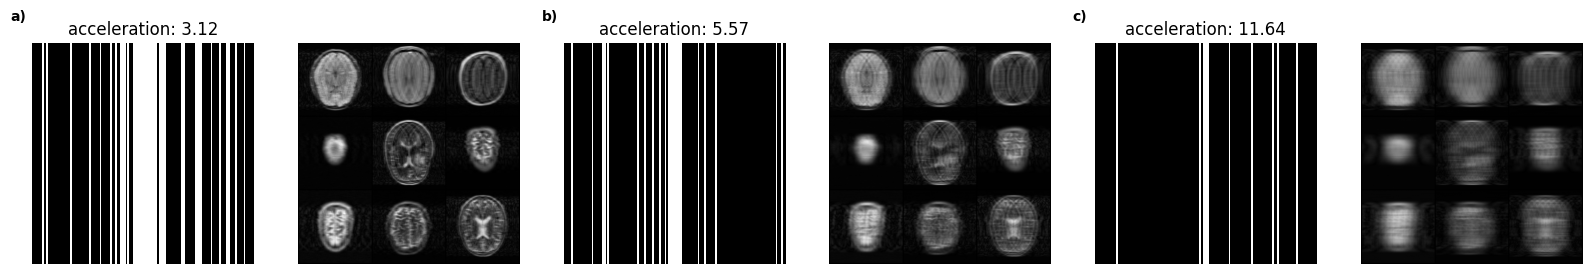
\includegraphics[width=\textwidth]{images/corruption_mask.png}
    \caption[K-Space Undersampling]{K-Space Undersampling: a) Sample of a K-Space undersampling mask with center fraction of 0.1 and a probability of 0.25 for the other frequencies, giving an effective acceleration of $\approx 3.12$. b) Effect of K-Space undersampling on samples from fastMRI dataset. While the low-frequency content is visibly intact, the undersampling of the higher frequencies causes aliasing artifacts, manifested as lines on the samples. These lines hint at the true aliases that would be generated for image space undersampling instead of randomized k-space undersampling.}
    \label{fig:kspacemasking}
\end{figure}

\section{Software Package}
In order to fully understand DDPMs it was decided to implement them from scratch instead of using repositories provided by the literature~\autocite{nichol2021improved} or by packages such as the Huggingface Diffusers library.~\autocite{huggingfacediffusers} The created repository is publicly accessible via GitHub and includes automatic documentation generation using Sphinx~\autocite{sphinx} and GitHub Actions~\autocite{githubactions}. Notable is also the useage of jaxtyping~\autocite{jaxtyping}, a library for type hinting tensor shapes. The repository and the documentation are accessible under the following links:
\begin{center}
    \hyperlink{https://github.com/liopeer/diffusionmodels}{\texttt{https://github.com/liopeer/diffusionmodels}}\\
    \hyperlink{https://liopeer.github.io/diffusionmodels/}{\texttt{https://liopeer.github.io/diffusionmodels/}}
\end{center}
The software package is based on PyTorch~\autocite{paszke2019pytorch} and provides model architectures as well as training utilities. These utilities include the possibility for 1. distributed training, 2. training logging and checkpointing, 3. mixed-precision training and inference, implemented using the following frameworks.
\begin{description}
    \item[Weights \& Biases] provides an API that allows logging the model training via their website (\hyperlink{https://wandb.ai/}{\texttt{https://\-wandb.ai/}}). The tool is free for students and academic researchers and automatically logs model configuration, gradients and hardware parameters in addition to user-specified logs, such as sample images, losses and inference times. When using git for versioning it also logs the most recent git commit, allowing to resume model training or to rerun an experiment with exactly the same code. When training models over several days it was very convenient to be able to observe the process from the smartphone and look at samples generated by the model.~\autocite{wandb}
    \item[PyTorch DDP (Distributed\-Data\-Parallel)] parallelizes model training by launching individual processes for each GPU, or it can even launch processes across different machines. Separate processes are necessary in order to enable true parallelism that avoids Python GIL (global interpreter lock). During initialization, the model is copied across the different GPUs and during training only the gradients are synchronized and averaged across the GPUs, therefore the optimizers essentially train a local model per each process. Gradient synchronization is automatically invoked by calling \texttt{loss.backward()}, but can be avoided by including forward and backward passes of the neural network in the \texttt{no\_sync()} content manager, which is useful when using gradient accumulation over several micro-batches, where the gradient synchronization would create unnecessary overhead. As part of DDP, PyTorch also offers \texttt{Distributed\-Sampler} (to be used with \texttt{Data\-Loader}), which splits mini-batches into micro-batches and assigns them to the respective processes. For models that use batch normalization layers, DDP also offers the module \texttt{SyncBatchNorm} and a function to recursively change all batch normalization layers to synchronized batch normalization. Synchronizing the batch normalization might be important for small micro-batch sizes or when the number of GPUs changes during training (e.g. continuing from a checkpoint).
    \item[PyTorch AMP (Automatic Mixed Precision)] provides a context manager and a function decorator that will convert certain operations to half-precision (16 bit), which gives a significant speedup for linear layers or convolutions, but keeps high precision for operations such as reductions. Half precision training might lead to underflow of gradients, because of the reduced value range and can be avoided by scaling the loss and therefore the gradients, while also inversely scaling the update step. AMP provides the \texttt{GradScaler} class for this purpose.
\end{description}